\section{The Metric Quad Ribbon}
\label{sec:quadribbon}

\plain{In brief: this is the flattening. Given accepted geometry, we must give every point a position on the page such that horizontal distance is true distance along the unrolled papyrus. Get this wrong by a few percent and the drift accumulates over metres of sheet until letters no longer line up with themselves; get the winding wrong and two different turns land on top of each other.}

\subsection{Probabilistic Winding Inference}
\label{sec:prob-winding}

Each disconnected mesh component has a continuously lifted cylindrical phase $q_i$, but that phase is known only up to an integer turn $k_c$. A maximum-support forest gives a coherent initial gauge, yet a forest necessarily discards its cycle-closing relations: one wrong heavy edge can shift an entire subtree while every relation inside that subtree remains satisfied. The current winding stage therefore treats the forest as an initializer rather than as truth.

\paragraph{A probabilistic field observation.} For an oriented triangle soup, let
\begin{equation*}
  g(x)=\frac{1}{4\pi}\sum_{f}\Omega_f(x)
\end{equation*}
be its generalized winding number, with $\Omega_f$ the signed solid angle of face $f$~\cite{jacobson2013winding}. Components are first orientation-voted against the umbilicus. At every sampled vertex $v_i$ we evaluate the field on both sides of the sheet,
\begin{equation*}
  m_i=\tfrac12\bigl(g(v_i+\epsilon n_i)+g(v_i-\epsilon n_i)\bigr),
  \qquad
  j_i=g(v_i-\epsilon n_i)-g(v_i+\epsilon n_i).
\end{equation*}
A clean, consistently oriented sheet has $j_i\simeq1$. A duplicate same-orientation shell tends toward two, an orientation cancellation toward zero. We therefore weight a sample by
$r_i=\exp[-\tfrac12((j_i-1)/0.35)^2]$ and discard $r_i<0.05$. The implementation chooses the exact boundary-edge reduction of Xie et al.~\shortcite{xie2026fast} when its measured work is affordable and otherwise uses the second-order fast expansion of Barill et al.~\shortcite{barill2018fast}, with exact triangles in the near field.

For component $c$, the field votes for its missing integer through the weighted median of $-m_i-q_i$. Its uncertainty is the larger of one turn and $1.4826$ times the weighted median absolute deviation; the one-turn epistemic floor is intentional, because an incomplete scroll field can look locally sharp while compressing the global range. Within each measured relation island, a positively sloped robust affine calibration maps the field cue into the forest gauge. A fit with fewer than three supported components, slope outside $[1/8,8]$, or $R^2<0.25$ contributes no unary.

\paragraph{MRF reconciliation.} Let $k_c$ be the integer correction for component $c$. Every admitted continuation or radial-order observation remains an individual pairwise factor with target $t_e$; contradictory factors are not averaged away. The optimized energy is
\begin{equation}
  \begin{aligned}
  E(k)={}&\sum_c \alpha_c\,\rho_{2.5}\!\left(\frac{k_c-\mu_c}{\sigma_c}\right)\\
       &+\sum_{e=(a,b)}\beta_e\,\left|(k_b-k_a)-t_e\right|\\
       &+\sum_{(c,\ell)\in\mathcal P}\gamma_{c\ell}\,[k_c=\ell],
  \end{aligned}
  \label{eq:winding-mrf}
\end{equation}
where $\rho$ is Huber, $(\mu_c,\sigma_c,\alpha_c)$ come from the calibrated field, and $\mathcal P$ is an optional sparse set of forbidden assignments. Continuations retain a modest preference over order factors, but the historical forest-priority offset is removed because it encoded an ordering artifact rather than evidence mass. Alpha--beta swap graph cuts~\cite{boykov2001fast} optimize residual labels in $[-2,2]$ around the current state; after a nonzero update the state is recentered and solved again, for at most four hierarchical rounds. The relation-island root is fixed. Output confidence is the sharpness of the local conditional label distribution with neighbouring MAP labels held fixed, not a claimed exact global marginal; sharpness below 0.35 is reported as unresolved.

\paragraph{Conflict penalties.} A second pass asks whether the current labels place spatially remote geometry in the same developed cell. Claims are keyed by relation island, axial bin, absolute integer turn, and wrapped-phase bin. Samples within $0.55$ local pitch are one physical claimant; only clusters separated by at least eight pitches and 48 voxels are mutually exclusive. The current test deliberately ignores ordinary two- and three-layer occupancy, which belongs to quadribbon layer handling, and targets only a cell with at least four claimant clusters. The claimant supported by the greatest mass of satisfied relations keeps the cell. A component may receive a forbidden $(c,k_c)$ assignment only if it loses in at least one such cell and wins in none. During the outer solve, every component not currently occupying a forbidden assignment is fixed, so the losing batch can use relations to the unchanged field without dragging that field with it. A band of eight turns around the base MRF prevents an integer cascade.

This outer pass does not currently work, and the way it fails is informative. The first unguarded experiment expanded the $4\times5\times5$ winding span from 14.13 to 32.41 turns over 24 exclusion rounds: forbidding an assignment is cheapest to satisfy by moving a component a whole turn away, so the penalties resolved collisions by inventing turns. Restricting them does not repair the underlying tension. A broad sweep counts 21,420 conflicting cells; winner- and context-lock variants reduce this to 11,099/10,214 while driving continuation/order satisfaction to 0.95789/0.66605 and 0.95580/0.80329 --- the exclusions are paid for out of the relations that produced the labels. Restricting attention to the four-claimant case leaves two cells and four losing claims; the one-bin variant clears both in four rounds using 20 forbidden assignments and preserves the 14.13-turn span, but creates 42 residual relation conflicts and raises MRF energy from 200.486 to 1,119.330, while requiring the loss in two cells makes no exclusion at all. A count of spatial collisions is simply a weaker measurement than a relation, and every configuration we tried either leaves the conflict or spends more relation evidence than the conflict is worth.

\paragraph{Standalone artifact.} \texttt{scroll\_ribbon --winding-only} stops before any ribbon graph or metric solve and writes topology-identical VMESH geometry with winding $U$, axial $V$, plus field, jump, label, confidence, and JSON sidecars. This separates the discrete labelling from everything downstream that could make a wrong label look visually smooth.

\subsection{From Mesh Pile to Ribbon}
\label{sec:fit}

The active executable takes a recursive pile of per-cube meshes and writes one staged result:
\begin{align*}
  \text{mesh soup}
  &\;\rightarrow\;\text{fit and metric solve}\;\rightarrow\;\text{untangle}
  \\
  &\;\rightarrow\;\text{metric re-solve}\;\rightarrow\;
  \text{layer bakes and composite}.
\end{align*}
Global geometric welding is omitted, and the feasibility of omitting it was measured before the path was built. On the $4\times5\times5$ pile, 100 per-cube meshes contain 783 raw geometry components; claims ownership and phase-continuation association reduce these to approximately 25 material candidates with saturated cube-seam continuation. The welded mesh, for comparison, yields 24. Cross-cube continuity is therefore obtainable as a fitted relation, and does not require two independently remeshed seam triangulations to agree as geometry.

\paragraph{Rows from slices.} The fit intersects the mesh soup with planes normal to the scroll axis. Mesh-edge identity chains the resulting intersections into \emph{row observations} --- chaining by shared edges rather than by endpoint proximity, since proximity is exactly the unreliable quantity here. Winding registration supplies continuously lifted cylindrical phase for those rows.

\paragraph{Continuation, and its limit.} Local continuation can close short discontinuities but must not span an entirely missing arc. Disjoint phase intervals are joined only when three conditions hold together: their angular gap is at most 1.3 radians, their axial supports overlap, and their radial change matches the local spiral pitch (within half a pitch). The third condition is the one doing the work --- it asks whether the junction \emph{continues the wrap} --- and without it, the first two would happily join a sheet to its own next turn. Gaps of 4.2 radians or more stay split for an evidence-backed pass. Branch lanes and delaminations are retained as parallel material candidates rather than averaged, since averaging two plies destroys both.

This continuation rule has a measured origin. Before it existed, one physical sheet tiled consecutive angular intervals as separate material islands: a chain of intervals with gaps of 0.36--1.19 radians across holes of 175--525 voxels, each individually plausible as a distinct island. The sheet was one sheet; the fit had simply had no vocabulary for saying so.

\subsection{Metric Projection}
\label{sec:metric}

Two experiments isolate complementary halves of metric parameterization, and we keep them separate deliberately: one establishes what a carried frame already determines, and the other establishes what independent observations can add.

\paragraph{Fixed-topology projection: no solver at all.} In the fixed-topology campaign, each row chain is oriented against the carried frame, assigned exact 3-D arclength $s$, and projected as
\begin{equation*}
  u_i = F(s_i + g_c),
  \qquad
  g_c = \operatorname{median}_{i\in c,\;|du/ds-1|\le0.15}(u_i^{\mathrm{seed}}-s_i),
\end{equation*}
where $F$ is a single reciprocal-integrated metric-rate map shared by the entire carried axis, and the per-chain offset $g_c$ is a robust median: only samples already locally metric to within 15\% vote on where their chain sits. Detached islands are placed rigidly through the monotone authoritative phase-to-$u$ map of the dominant component. No recomputed principal-angle fallback may place an unanchored island, because a fallback that guesses is indistinguishable in the output from a measurement that knows.

On $4\times5\times5$ this path needs no numerical solver, preserves all 4,033,291 faces, and runs in 9.6 seconds. Its value is as a control: it proves that exact metric projection plus authoritative phase placement --- with no optimization anywhere --- already recovers every user-marked dropout that another evidenced layer covers.

\paragraph{Robust consistency: where independent observations disagree.} The pre-weld fit contains real cracks and contacts that a fixed carried topology does not. Here we solve their consistency explicitly rather than accumulating local corrections, which is the difference between reconciling measurements and propagating an error. For scalar $u$ values $x$, rows encode observed differences $d_i$:
\begin{equation*}
  \min_x \sum_{i\in\mathcal R} w_i\,\rho_{c_i}\!\left((x_{a_i}-x_{b_i})-d_i\right),
\end{equation*}
where $\rho$ is Huber. \emph{Metric rows} ask consecutive samples to advance by their measured arclength; \emph{vertical and face-contact rows} ask for zero drift; and \emph{crack ties} close an evidenced fissure --- admitted only where neither facing side already carries a face tie, so a crack cannot be closed twice by two different mechanisms. One pin per component fixes each null space.

Normal equations are assembled into lower-triangular sparse form and solved by TAUCS supernodal multifrontal Cholesky, with at most three IRLS rounds recomputing exact residual weights. The $4\times5\times5$ system has 2.04 million unknowns and 12.2 million nonzeros and factors in 8--11 seconds. Its 28,597 crack ties reduce visible $\pm20$--25-pixel slips to approximately $\pm1.3$; texture cross-correlation measures a median sheet-seam shift of 3 pixels rather than 10--25. Island placement is then repeated against the solved, coherent $u$ field before a global non-negative re-zero.

Running island placement twice is not redundancy. The phase-to-$u$ map used on the first pass is built from the carried $u$, which at the inner turns is compressed and locally non-monotone; placements derived from it collapse onto a plateau. Rebuilding the map from the \emph{solved} field and re-placing is what recovers inner-turn order.

\paragraph{Neither solver owns identity.} This is the invariant that makes the two experiments composable. Solver-free projection establishes what the carried metric frame already determines; IRLS is used only where independent pre-weld observations supply residual constraints. Neither chooses winding identity. That authority stays with continuous phase and the assembly graph, which is what prevents a least-squares residual from purchasing a wrap change.

\begin{figure*}[t]
  \centering
  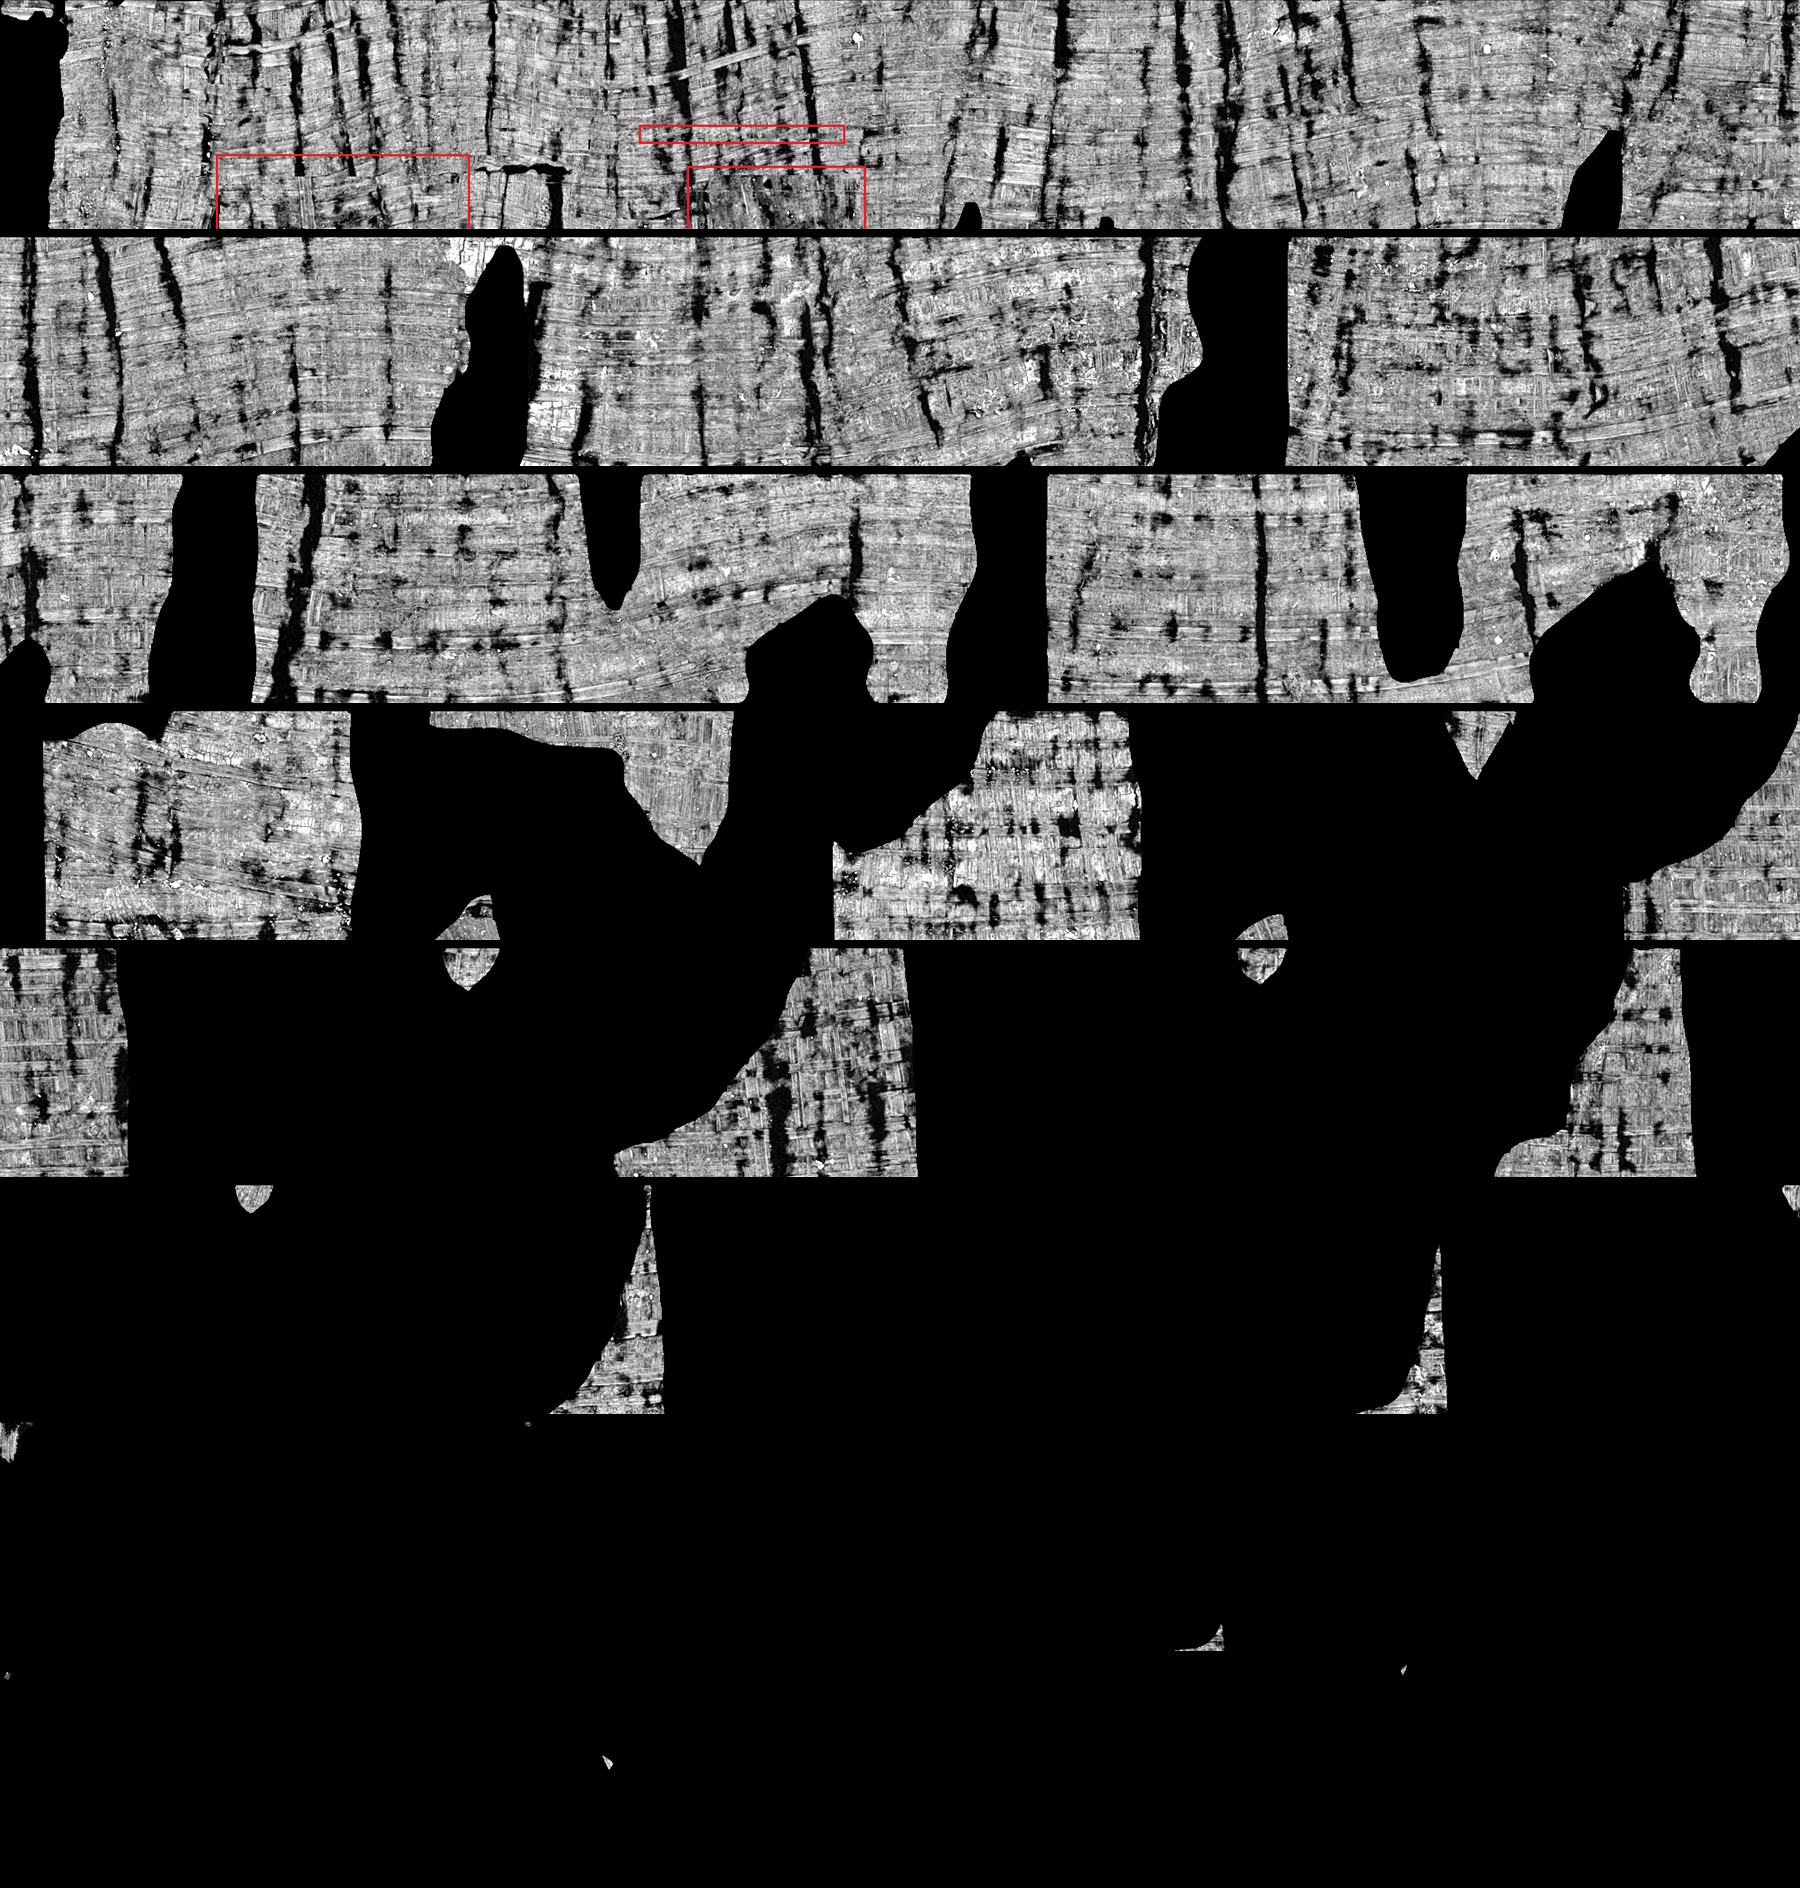
\includegraphics[width=0.82\linewidth]{figures/quadribbon_4x5x5_page.jpg}
  \caption{The $4\times5\times5$ fixed-topology metric composite, reformatted from its native $31{,}127\times508$ ribbon into reading rows. All 4,033,291 faces are conserved. Red boxes mark the previously identified dropout sites; evidenced secondary layers now cover them. Black areas remain unsupported rather than being presented as papyrus.}
  \Description{A grayscale multi-row papyrus texture with fibre structure, cracks, explicit black unsupported regions, and a few red boxes around formerly missing strips.}
  \label{fig:metric-sheet}
\end{figure*}

\subsection{Reading the Result}

The final image is also the strongest available test of the parameterization, and it is a physical test rather than a numerical one. For each texel of the developed $(u,v)$ image we sample CT intensity at the corresponding surface point. If $u$ is a correct developed arc length, the two papyrus fibre families remain continuous across the page; a wrong parameterization shears, duplicates, or breaks them. Dark bands that persist coherently across rows are cracks and damage rather than parameterization artifacts. On synthetic spirals with known geometry, the local solver tracks analytic arc length to within a fraction of a percent across all turns.

The $10\times10\times10$ region (Fig.~\ref{fig:sheet-10x-hybrid}) is currently unwrapped by composing the two campaigns directly: the solid connected quad ribbon supplies topology and a first-guess parameterization, and the TAUCS consistency solve then re-fits $u$ for constant arclength across $v$ on that fixed topology --- 16.4 million unknowns, 98.7 million nonzeros, three IRLS rounds, 25 minutes. The re-fit removes the inter-wrap drift responsible for earlier waved composites: contact residuals collapse from $p10/p90 = -1304/{+}324$ pixels to $-2.5/{+}2.5$, while the row metric is essentially untouched ($|du/ds-1|$ mean 0.058 before and after). That combination --- a hundredfold improvement in cross-wrap consistency at no cost in along-row metric --- is the signature of a drift that was a frame error rather than a measurement error. The bake samples the complete masked CT volume; for context, the original run of this ribbon was missing 728 of 1,728 RAW cubes.

\begin{figure*}[t]
  \centering
  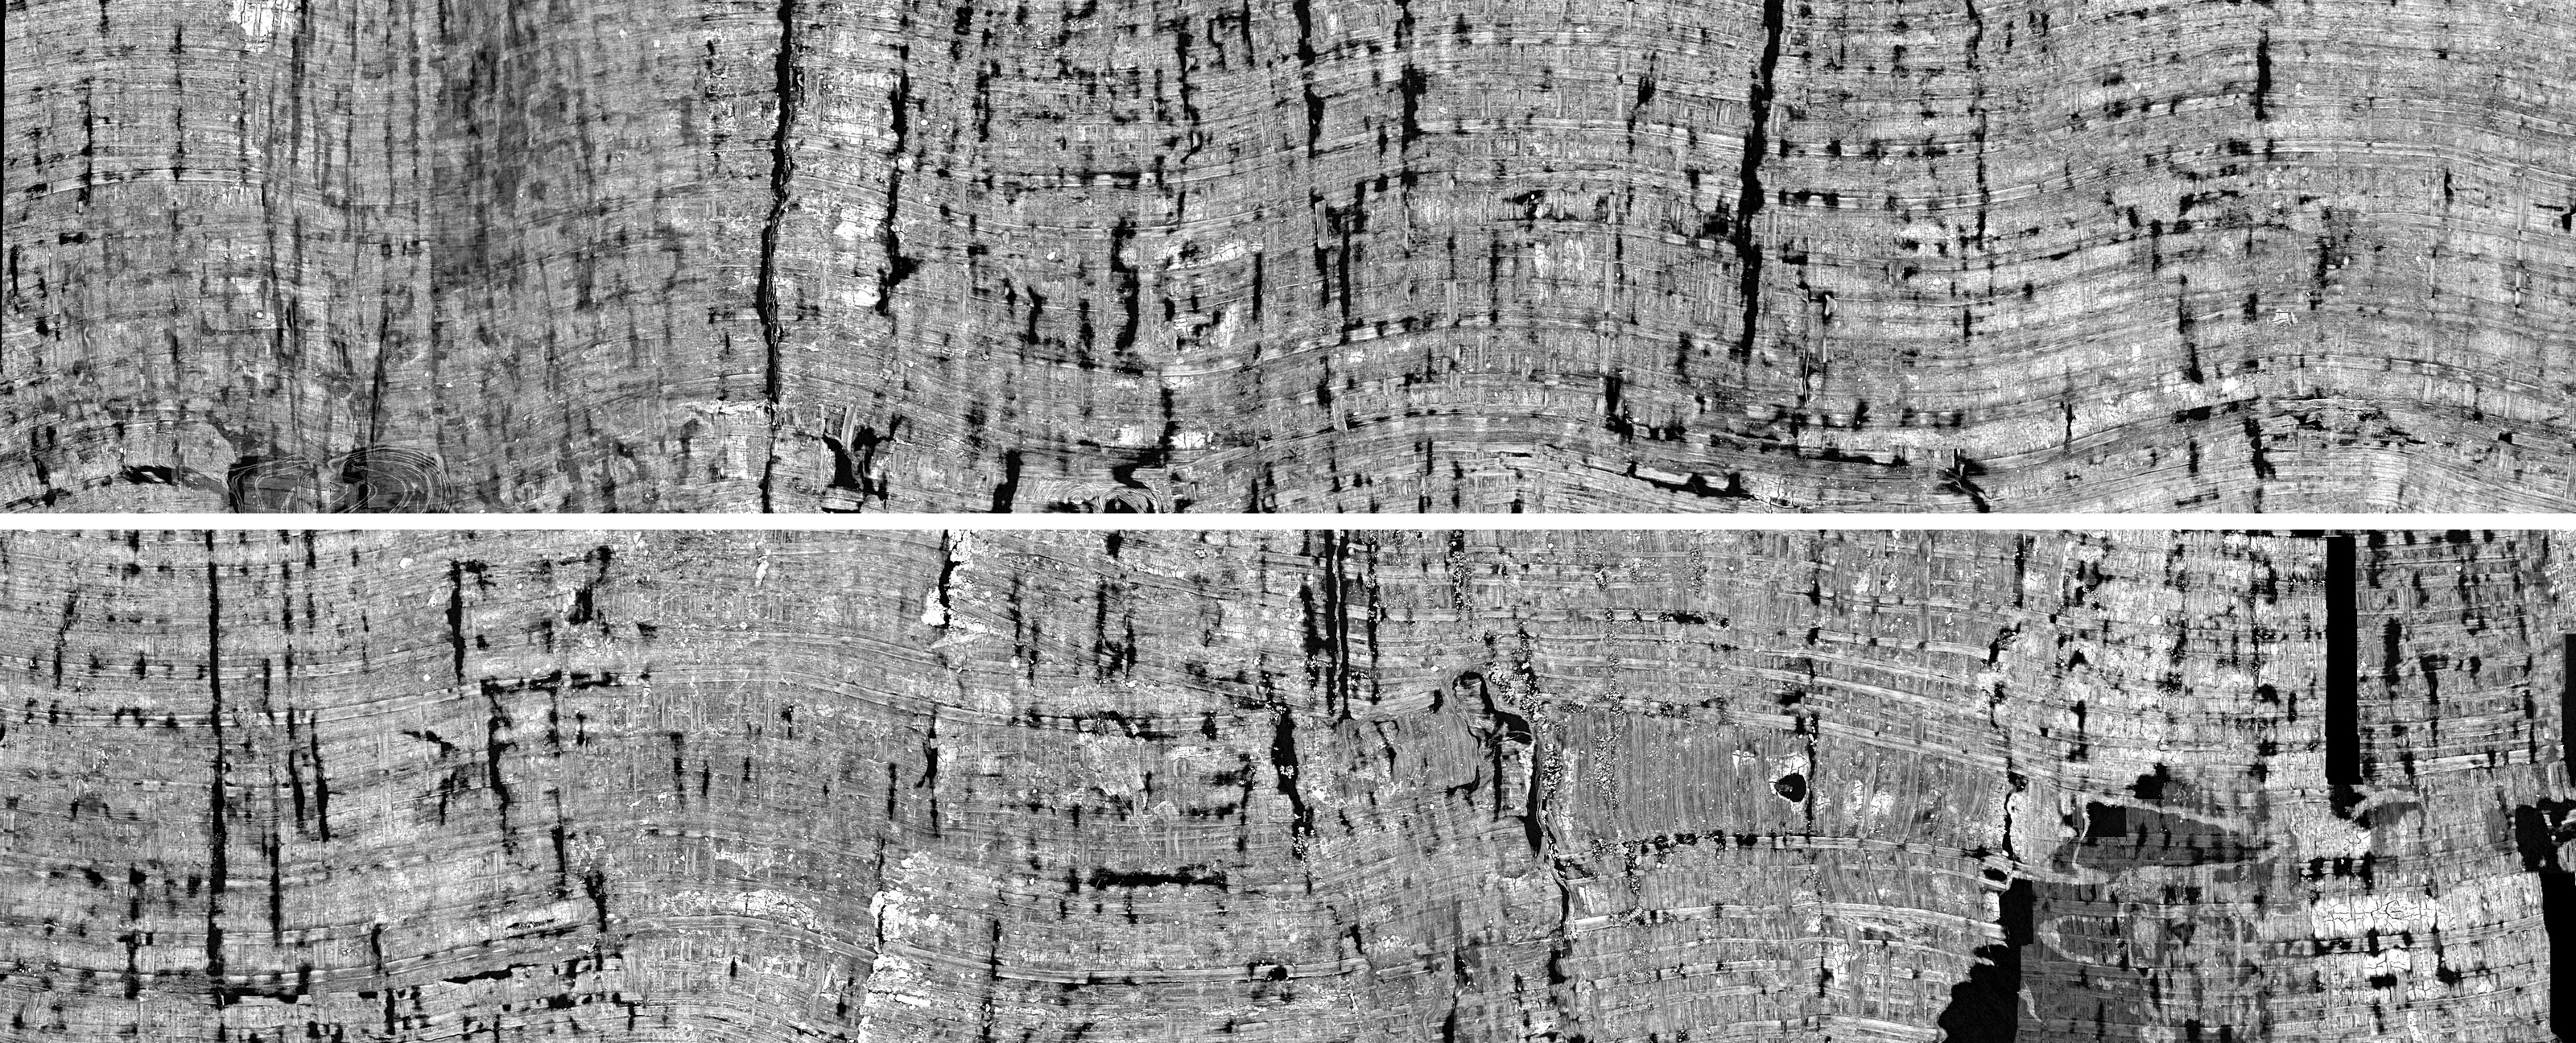
\includegraphics[width=0.82\linewidth]{figures/quadribbon_10x10x10_hybrid_strip.jpg}
  \caption{A $10\times10\times10$ sheet: the central 12{,}800-pixel span of the $33{,}338\times1{,}276$ composite, reformatted into two reading rows. The solid quad ribbon supplies connected topology; the constant-arclength re-fit supplies the metric ($\pm1300\rightarrow\pm2.5$-pixel contact residuals). Dark regions are cracks and unsupported material, not fill.}
  \Description{Two stacked wide rows of grayscale papyrus texture with continuous horizontal fibre structure, vertical cracks, and small dark voids.}
  \label{fig:sheet-10x-hybrid}
\end{figure*}

\subsection{Integration State}
\label{sec:integration-state}

The consolidated command is \texttt{quadribbon <mesh\_dir> <out\_dir>}. It writes the concatenated soup, fitted ribbon, first metric solution, untangled geometry, second metric solution, layer manifests, RAW bakes, composite, label image, and per-stage logs. Stage artifacts are resumable, and production constants --- axis, pitch, CT source, bake window, dark threshold --- come from one frozen configuration rather than from tuning flags on the command line.

At the current snapshot, all module self-tests pass and the canonical $4\times5\times5$ run from the pre-weld pile completes end to end. The fixed-topology and solid-ribbon campaigns reported in this section and the next are the quantitative evidence for parameterization, attachment, and compositing; we do not relabel them as output of the integrated command. Larger canonical pre-weld piles have not yet traversed this exact sequence.
